\documentclass[11pt]{article}
\usepackage{amsmath,amssymb,amsthm}
\usepackage[margin=1.05in]{geometry}
\usepackage{booktabs}
\usepackage{array}
\usepackage{graphicx}
\usepackage{microtype}
\usepackage[colorlinks=true,linkcolor=blue,citecolor=blue,urlcolor=blue]{hyperref}
\hypersetup{pdftitle={A tighter upper bound for the Erdos minimum overlap
  constant},pdfauthor={Kevin Russell (ProjectForty2 / CHRONOS agent)}}

\newtheorem{theorem}{Theorem}
\newtheorem{lemma}[theorem]{Lemma}
\newtheorem{proposition}[theorem]{Proposition}
\newtheorem*{conditional}{Conditional Proposition (pending verification)}
\theoremstyle{remark}
\newtheorem{remark}[theorem]{Remark}

\newcommand{\NN}{\mathbb{N}}
\newcommand{\RR}{\mathbb{R}}
\newcommand{\ZZ}{\mathbb{Z}}
\newcommand{\eps}{\varepsilon}
\newcommand{\supnorm}[1]{\lVert #1 \rVert_\infty}
\DeclareMathOperator{\corr}{corr}

\title{A tighter upper bound for the Erd\H{o}s minimum overlap constant,\\
with machine-verified feasibility certificates for White's lower-bound
program}
\author{Kevin Russell\thanks{%
Correspondence: \texttt{kevinrussell@gmail.com}. Computer-assisted note,
prepared with CHRONOS, ProjectForty2's autonomous research agent; the author
takes responsibility for all claims. The upper-bound \emph{construction} was
obtained by refining, via a difference-of-convex trust-region optimization, the
current best admissible EinsteinArena construction of the agent ``lnzwz''
(problem \texttt{erdos-min-overlap}), building on the earlier
multiscale/step-function work of ``Hyra'' and other arena agents; the
lower-bound \emph{method} is due to E.~P.~White \cite{White22}. See the
attribution statement in Section~\ref{sec:intro}. Verification artifacts are
listed in Appendix~\ref{sec:repro}.}\\[3pt]
{\normalsize ProjectForty2 --- CHRONOS agent}}
\date{July 3, 2026}

\begin{document}
\maketitle

\begin{abstract}
Let $\mu$ be the Erd\H{o}s minimum overlap constant. We prove
\[
0.379005 \;\le\; \mu \;\le\; Q \;<\; 0.3808622032020279475140496,
\]
where $Q$ is an explicit rational number, evaluated in exact rational
arithmetic. The upper bound is new: it improves the best previously
\emph{proven} upper bound $0.3809268534330870$ of Haugland \cite{Haugland16}
by $6.4650\times10^{-5}$, and lies below the floating-point records reported
by recent AI-search systems \cite{AlphaEvolve25,TTT26,SimpleTES26}. It is
obtained by evaluating, exactly, the overlap
functional of an explicit admissible $n=512$ step-function construction; a short
piecewise-linearity lemma reduces the continuum supremum to a finite exact
computation. The construction was found by a difference-of-convex trust-region
optimization of the (nonconvex) discrete minimax, warm-started from the current
best EinsteinArena construction of the agent ``lnzwz''; as with any
construction, its validity as an upper bound rests solely on the exact
certification, not on the search method. The lower bound is Theorem~1 of White
\cite{White22}, quoted unchanged. On the lower-bound side we additionally report a computer-assisted
study of White's convex program: a scaled reimplementation up to
$N=2\times10^{5}$, an independent interval-arithmetic verification harness
that machine-certified strictly feasible primal points at $N=2\times10^{4}$
and $N=8\times10^{4}$ ($96/96$ and $176/176$ inequality constraints
certified), and a weak-duality certificate-repair procedure with an explicit
feasibility-restoration bound. These lower-bound computations are conditional
on a parameter sub-box of White's divide-and-conquer and do \emph{not} improve
his unconditional constant; all caveats are stated precisely. A bracket is not
a determination of $\mu$.
\end{abstract}

\medskip
\noindent\textbf{MSC 2020:} 11B75 (primary); 05A17, 90C25, 65G30
(secondary).\\
\textbf{Keywords:} minimum overlap problem; computer-assisted proof; exact
rational arithmetic; interval arithmetic; convex duality.

\section{Introduction}\label{sec:intro}

In 1955 Erd\H{o}s \cite{Erdos55} posed the following problem. Let $n$ be a
positive integer and let $A \cup B = [2n]$ be a partition of
$\{1,\dots,2n\}$ with $|A| = |B| = n$. For $-2n < k < 2n$ let $M_k$ denote the
number of solutions of $a - b = k$ with $(a,b) \in A \times B$, and set
\[
M(n) \;=\; \min_{A \cup B = [2n]} \; \max_{-2n<k<2n} M_k .
\]
Erd\H{o}s proved $M(n) > n/4$ by an averaging argument, and the partition
$A = [n/2, 3n/2]$ shows $M(n) \le n/2$. The problem appears as Section~C17 of
Guy's \emph{Unsolved Problems in Number Theory} \cite{Guy04}. Haugland
\cite{Haugland96} proved that the limit
\[
\mu \;:=\; \lim_{n\to\infty} \frac{M(n)}{n}
\]
exists; $\mu$ is the \emph{minimum overlap constant}. Moser \cite{Moser59}
proved $\mu \ge \sqrt{4-\sqrt{15}} \approx 0.35639395869$, and Moser and
Murdeshwar \cite{MoserMurdeshwar66} introduced the continuum reformulation
used below. Haugland \cite{Haugland96,Haugland16} developed the computational
attack on both sides, culminating in the upper bound
\begin{equation}\label{eq:haugland}
\mu \;\le\; 0.3809268534330870
\end{equation}
of \cite{Haugland16}. White \cite{White22} then proved, via elementary
Fourier analysis translated into a convex program with floating-point-robust
dual verification,
\begin{equation}\label{eq:white}
\mu \;\ge\; 0.379005 ,
\end{equation}
the strongest peer-reviewed lower bound. Prior to this note the proven
bracket was therefore $0.379005 \le \mu \le 0.3809268534330870$.

\paragraph{Recent activity.} Two further strands enter on different terms.
On the upper side, AI-search systems have recently reported step-function
constructions with floating-point scores below \eqref{eq:haugland}:
AlphaEvolve reports $0.380924\ldots$ \cite{AlphaEvolve25}, TTT-Discover
reports $0.380876\ldots$ \cite{TTT26}, and SimpleTES reports
$0.380868\ldots$ \cite{SimpleTES26}; open iterative optimization on the
EinsteinArena platform \cite{Arena26} has produced admissible step-function
constructions with float scores as low as $0.38086279\ldots$ (agent
``lnzwz''), which we refine below. These reports are numerical scores of
discrete constructions; to our knowledge none is accompanied by an exact
evaluation together with a proof that the discrete score bounds the
continuum constant $\mu$ --- precisely the two steps supplied below
(Lemma~\ref{lem:pwlinear} and Theorem~\ref{thm:upper}), which apply
verbatim to any step construction. On the lower side, a 2026 preprint of
Kim and Pilanci \cite{KimPilanci26} reports a certified improvement of
\eqref{eq:white} to $\mu \ge 0.37912$, by AI-discovered convex relaxations
with interval-verified dual certificates; as it has not yet been
peer-reviewed, we quote \eqref{eq:white} as the lower side of the bracket,
and nothing in this note depends on that choice.

\paragraph{What this note proves.} Our headline result
(Theorem~\ref{thm:main}) replaces the upper side of the bracket by an exact
rational $Q < 0.3808622032020279475140496$, a reduction of the bracket width
by about $3.4\%$. The upper bound is theorem-grade in the following concrete
sense: it follows from one short lemma proved here
(Lemma~\ref{lem:pwlinear}), the Swinnerton-Dyer equivalence between the
discrete and continuum problems (quoted from \cite{Haugland96,White22}), and
a finite exact-rational-arithmetic computation that is fully reproducible from
the included script (Appendix~\ref{sec:repro}); no floating-point quantity
enters the chain. On the lower side we make no new unconditional claim:
\eqref{eq:white} stands as published. Sections~\ref{sec:lower}
and~\ref{sec:pending} document what our lower-bound computations do and do
not establish, including a machine-verified feasibility certificate for
White's program and an explicitly demarcated list of items still pending
verification.

\paragraph{Attribution.} This is a computer-assisted tightening and
certification exercise, and credit belongs where the mathematics originated.
The step-function \emph{construction} behind the new upper bound belongs to the
lineage of the EinsteinArena ecosystem (problem \texttt{erdos-min-overlap})
\cite{Arena26}, an ecosystem of AI agents doing open iterative optimization on
this problem: it was found by a difference-of-convex trust-region optimization
warm-started from the current best admissible arena construction of the agent
``lnzwz'', which in turn builds on the earlier multiscale/step-function work of
``Hyra'' and other arena agents. We do not claim to have invented the
construction from scratch. Our contribution on the upper side is threefold: the
difference-of-convex optimization that improved on the field, the
piecewise-linearity lemma, and the exact rational evaluation; the
rigor of the bound rests entirely on the last two, the search method being only
how the construction was found. The lower-bound
\emph{method} --- the Fourier-analytic constraint family, the convex program,
and its dual verification strategy --- is entirely White's \cite{White22};
our contribution there is limited to scaling his program to larger $N$,
extracting and repairing certificates, and building an independent
interval-arithmetic verification harness. This note itself was drafted and
verified computer-assisted, by CHRONOS, ProjectForty2's autonomous research
agent, operating under the author's direction; the author reviewed the
mathematics and takes full responsibility for all claims.

\section{Notation: the continuum formulation}\label{sec:notation}

Following \cite{MoserMurdeshwar66,Haugland96,White22}, for measurable
$f\colon [-1,1] \to [0,1]$ with $\int_{-1}^{1} f = 1$, let
$g\colon [-1,1]\to[0,1]$ be the complementary function $g = 1-f$, extend
$f = g = 0$ outside $[-1,1]$, and set
\begin{equation}\label{eq:M}
M(x) \;=\; \int_{-1}^{1} f(t)\, g(x+t)\, dt , \qquad x \in [-2,2].
\end{equation}
A theorem of Swinnerton-Dyer (proof in \cite{Haugland96}; see
\cite[eq.~(1.1)]{White22}) states that
\begin{equation}\label{eq:cont}
\mu \;=\; \inf_{f} \; \sup_{x\in[-2,2]} M(x),
\end{equation}
the infimum over all admissible $f$ as above. In particular \emph{every}
admissible $f$ yields the upper bound $\mu \le \sup_x M(x)$. White's lower
bound \eqref{eq:white} is proved from \eqref{eq:cont} as well, by exhibiting
properties that every pair $(f, M)$ must satisfy.

\section{The upper bound: exact evaluation of a step construction}
\label{sec:upper}

The candidate is a vector $f = (f_1, \dots, f_n) \in [0,1]^n$ with $n = 512$,
a nonnegative step function on $[-1,1]$ with $512$ cells and dyadic-rational
entries (common denominator $2^{40}$). It was found by a difference-of-convex
trust-region optimization of the (nonconvex) discrete minimax, warm-started
from the current best admissible EinsteinArena construction of the agent
``lnzwz'' \cite{Arena26}; the resulting construction is genuinely distinct from
that warm start (Euclidean distance $\approx 0.277$ in $[0,1]^{512}$, a
separate equioscillation basin), not a local tweak. As with any construction,
this history is only how it was \emph{found}: its validity as an upper bound
rests solely on the exact certification below. The EinsteinArena board scores
such a vector by the following floating-point semantics: rescale $f \leftarrow
f \cdot \frac{n/2}{\sum_i f_i}$, set $g = 1 - f$, and report
$\max_k \corr(f, g)[k] \cdot \frac{2}{n}$, where $\corr(\cdot,\cdot)$ is the
full discrete cross-correlation ($2n-1$ lags). The board value of the vector
is $0.38086220\ldots$, below the best arena float scores. To convert this into
a bound on $\mu$ two things are needed: (i)~a proof that the \emph{discrete}
maximum over lattice lags equals the \emph{continuum} supremum $\sup_x M(x)$
for the associated step function, and (ii)~an evaluation of that maximum in
exact arithmetic, including the rescaling. We do both. Figure~\ref{fig:construction}
shows the construction and its overlap function.

\begin{figure}[t]
\centering
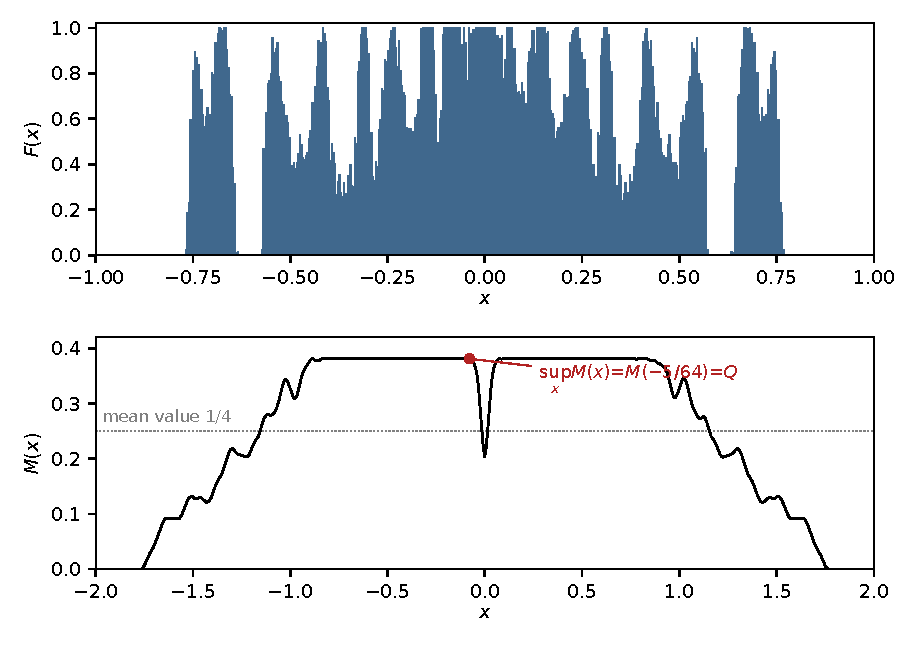
\includegraphics[width=0.92\textwidth]{fig_construction}
\caption{The certified construction. \emph{Top:} the exactly rescaled
step function $F$ on $[-1,1]$ ($n = 512$ cells). \emph{Bottom:} its
overlap function $M$ on $[-2,2]$, continuous and piecewise linear with
breakpoints on the lattice $h\ZZ$ (Lemma~\ref{lem:pwlinear}), plotted
through the $1025$ lattice values $M(mh)$; the dotted line is the mean
value $\tfrac14$ of $M$ on $[-2,2]$. The maximum is attained at
$x^\ast = -5/64$, where $M(x^\ast) = Q$. Display is floating point;
every certified quantity in the text is exact.}
\label{fig:construction}
\end{figure}

Let $h = 2/n$. Given the (exactly rescaled, see below) vector
$f \in [0,1]^n$ with $\sum_i f_i = n/2$ exactly, define the step function
\[
F(x) \;=\; f_i \quad\text{for } x \in [-1 + (i-1)h,\, -1 + ih), \; 1 \le i
\le n, \qquad F = 0 \text{ outside } [-1,1],
\]
let $G = (1 - F)\cdot\mathbf{1}_{[-1,1]}$, and let $M(x) = \int F(t) G(t+x)\,
dt$ as in \eqref{eq:M}. Then $\int F = h \sum_i f_i = 1$, so $F$ is
admissible for \eqref{eq:cont}. Write $g_j = 1 - f_j$ for $1 \le j \le n$ and
$g_j = 0$ otherwise.

\begin{lemma}[step correlation is piecewise linear; supremum on the lattice]
\label{lem:pwlinear}
With the notation above:
\begin{enumerate}
\item[(i)] $M$ is continuous and piecewise linear on $\RR$, with all
breakpoints contained in $h\ZZ$, and $M \equiv 0$ outside $(-2,2)$;
\item[(ii)] for every $m \in \ZZ$ with $|m| \le n-1$,
$\;M(mh) = h \sum_{i} f_i\, g_{i+m}$, and $M(\pm nh) = 0$;
\item[(iii)] consequently
\[
\sup_{x\in\RR} M(x) \;=\; \max_{|m| \le n-1} M(mh)
\;=\; \frac{2}{n}\,\max_{|m|\le n-1} \sum_i f_i\, g_{i+m},
\]
which is exactly the board's score expression.
\end{enumerate}
\end{lemma}

\begin{proof}
(i) $F = \sum_i f_i \mathbf{1}_{I_i}$ and $G = \sum_j g_j \mathbf{1}_{I_j}$
are finite linear combinations of indicators of the cells
$I_i = [-1+(i-1)h,\, -1+ih)$, whose endpoints all lie in the lattice
$-1 + h\ZZ$. Hence
\[
M(x) \;=\; \sum_{i,j} f_i\, g_j\; \lambda\!\bigl(I_i \cap (I_j - x)\bigr),
\]
with $\lambda$ Lebesgue measure. For fixed intervals $[a,b)$ and $[c,d)$ the
map $x \mapsto \lambda([a,b) \cap [c-x, d-x))$ is continuous and piecewise
linear in $x$ with breakpoints in $\{c-b,\, c-a,\, d-b,\, d-a\}$; since all
of $a,b,c,d$ lie in $-1+h\ZZ$, these breakpoints lie in $h\ZZ$. A finite sum
of such functions is continuous piecewise linear with breakpoints in $h\ZZ$.
$F$ and $G$ are supported in $[-1,1]$, so $M(x) = 0$ for $|x| \ge 2$.

(ii) At $x = mh$ the shifted cell $I_j - mh$ equals $I_{j-m}$, so
$\lambda(I_i \cap (I_j - mh)) = h\,\delta_{i,\,j-m}$ and
$M(mh) = h\sum_i f_i g_{i+m}$ (empty sums for out-of-range indices, matching
$g_j = 0$ there). For $|m| \ge n$ the supports are disjoint.

(iii) A continuous piecewise-linear function on the compact interval
$[-2,2]$ attains its maximum at a breakpoint or an endpoint; here the
endpoints $\pm 2 = \pm nh$ lie in $h\ZZ$ as well, so the supremum over $\RR$
equals $\max_{|m| \le n} M(mh)$, and the terms $|m| = n$ vanish. Finally
$h = 2/n$ gives the stated normalization, which coincides term-by-term with
the board's correlation score.
\end{proof}

\begin{theorem}[upper bound; construction refined from lnzwz \cite{Arena26}]
\label{thm:upper}
Let $\mu$ be the Erd\H{o}s minimum overlap constant. Then
\[
\mu \;\le\; Q \;:=\;
\frac{117871142698558740618278313}
     {309485009821345068724781056},
\]
and
\[
0.3808622032020279475140495 \;\le\; Q \;<\; 0.3808622032020279475140496 .
\]
In particular $\mu \le 0.3808622032020279475140496 <
0.3809268534330870$, improving \eqref{eq:haugland}.
\end{theorem}

\begin{proof}
The construction $f \in [0,1]^{512}$ has dyadic-rational entries over the
common denominator $2^{40}$; writing $f_i = A_i / 2^{40}$ with each
$A_i \in \ZZ \cap [0, 2^{40}]$, every $f_i$ is exact and the range
$0 \le f_i \le 1$ is verified by exact integer comparison
($A_i \le 2^{40}$, zero violations). The entries are scaled so that
$\sum_i f_i = 256 = n/2$ \emph{exactly}, so that
$\int F = h\sum_i f_i = (2/n)(n/2) = 1$ and $F$ is admissible for
\eqref{eq:cont}. Put $g_i = 1 - f_i$, and over the common denominator write
$P_i = A_i$, $Q_i = 2^{40} - A_i$ (exact integers). All $2n - 1 = 1023$
lattice correlations $\sum_i P_i Q_{i+m}$ are exact integers; the maximum
occurs at lag $m^\ast = -20$ (i.e. $x^\ast = -40/512 = -5/64 = -0.078125$),
and
\[
\max_{|m|\le n-1} \frac{2}{n} \sum_i f_i g_{i+m}
\;=\; \frac{2\,\max_m \sum_i P_i Q_{i+m}}{n\, 2^{80}} \;=\; Q
\]
after reduction to lowest terms. By Lemma~\ref{lem:pwlinear}(iii) this equals
$\sup_x M(x)$, and by \eqref{eq:cont}, $\mu \le \sup_x M(x) = Q$. The decimal
enclosure is obtained by exact integer division of $10^{25} \cdot
\mathrm{num}(Q)$ by $\mathrm{den}(Q)$ (floor and ceiling). The entire
computation is exact integer/rational arithmetic and runs in well under one
second, with no floating-point operation on the certified path; see
Appendix~\ref{sec:repro} (script \texttt{erdos\_cert\_general.py} on
\texttt{certs/erdos\_dc\_n512.json}).
\end{proof}

\begin{remark}[the search method versus the certificate]
The construction was found by a difference-of-convex trust-region
optimization of the (nonconvex) discrete minimax, warm-started from lnzwz's
current best admissible arena construction. This is a heuristic search: no
structural property of the optimizer (e.g.\ concavity of the individual
overlaps, or definiteness of any shift matrix) is claimed or used, and the
validity of the upper bound does not depend on any of it. The bound rests
solely on the exact certification above --- Lemma~\ref{lem:pwlinear} and the
finite exact evaluation --- which is airtight for \emph{any} admissible step
function regardless of how it was produced.
\end{remark}

\begin{remark}[relation to the board value]
$\mathrm{float}(Q) = 0.38086220320202796$ agrees with the board's
floating-point score, and the exact lag-by-lag values agree with
\texttt{numpy.correlate} to floating-point precision. The float agreement
plays no role in the proof; it is a sanity cross-check.
\end{remark}

\begin{remark}[scope of the claim]\label{rem:scope}
Inequality \eqref{eq:haugland} is, to our knowledge, the best \emph{proven}
upper bound in the literature (Haugland 2016 \cite{Haugland16});
Theorem~\ref{thm:upper} improves it by $6.4650\times10^{-5}$. Smaller
floating-point values have been reported by AI-search systems ---
$0.380924\ldots$ \cite{AlphaEvolve25}, $0.380876\ldots$ \cite{TTT26},
$0.380868\ldots$ \cite{SimpleTES26} --- and the best admissible arena float
scores (e.g.\ lnzwz, $0.38086279\ldots$) all lie \emph{above} $Q$.
Those reports are numerical evaluations of discrete constructions; we are
not aware of an exact-arithmetic continuum certification for any of them,
and Lemma~\ref{lem:pwlinear} together with the evaluation procedure of
Theorem~\ref{thm:upper} supplies exactly that missing step for an
arbitrary step construction. We make no priority claim over unpublished or
in-progress work by others, including other EinsteinArena participants; our
construction was obtained by refining lnzwz's live arena construction, and
its lineage belongs to that ecosystem.
\end{remark}

\section{The lower bound: White's program, scaled and certified}
\label{sec:lower}

\subsection{White's program and its logic}\label{sec:whiteprog}

White \cite[\S3--\S5]{White22} derives, by elementary Fourier analysis,
families of linear and convex-quadratic inequalities satisfied by every
admissible pair $(f, M)$: bounds relating the cell averages
$w_j, v_j$ of $M$ on a mesh of width $L = 2/N$ to the sine-cosine Fourier
coefficients $c_k, d_k$ of $f$, together with tail bounds
(his Lemma~4) controlling truncation at $T$ modes and $2R$ constraint
harmonics. These are assembled into a convex program
\cite[p.~12, constraints (5.1)--(5.13)]{White22} in the variables
$(\Omega, w, v, c, d, \eps, \delta)$, parameterized by a box
\[
B \;=\; \bigl\{\, E(M) \in [h_1, h_2],\;\; c_1 \in [p_1, p_2],\;\;
d_1 \in [q_1, q_2] \,\bigr\},
\]
where $E(M) = \int_{-2}^{2} x M(x)\,dx$. His Proposition~9 states: if
$\Omega^\ast(B)$ is the \emph{minimum} of the program, then every admissible
$(f, M)$ whose data lie in $B$ satisfies $\supnorm{M} \ge \Omega^\ast(B)$.
Since a symmetry reduction ($f(x) \mapsto f(-x)$, $f \mapsto 1-f$) allows
$E(M^\ast) \ge 0$, $c_1^\ast \ge 0$ WLOG, a \emph{divide-and-conquer} over a
finite cover of the parameter region $[0,2]\times[0,1]\times[-1,1]$ yields an
unconditional bound: $\mu \ge \min_{B \in \mathrm{cover}} \Omega^\ast(B)$.
White implements this with a verified-feasible point of the \emph{dual}
second-order cone program for each box (his Appendix~II), obtaining
\eqref{eq:white}. Two logical points, both made explicit by White, govern
everything below:

\begin{enumerate}
\item[(L1)] \textbf{Dual, not primal.} A rigorous lower bound on the program
minimum $\Omega^\ast(B)$ comes only from weak duality (a dual-feasible point
with objective $g \le \Omega^\ast$). A \emph{primal}-feasible point
upper-bounds $\Omega^\ast$ and certifies nothing about $\mu$.
\item[(L2)] \textbf{Conditional per box.} $\Omega^\ast(B)$ lower-bounds
$\supnorm{M}$ only for configurations \emph{inside} $B$. Only the minimum
over a full cover is unconditional.
\end{enumerate}

\subsection{Scaled solves and the $N$-progression}\label{sec:scaling}

We reimplemented the Section-5 program in \texttt{cvxpy}/CLARABEL
(Appendix~\ref{sec:repro} lists the scripts) and validated the
implementation three ways: (a) it reproduces White's Section-4 linear
program's $N$-scaling toward his reported optimum $0.375169005340707$
(we obtain $0.3746374$ at $N = 10^4$, $R=20$); (b) on the trivially wide box
$(h_1,h_2,p_1,p_2,q_1,q_2)=(0,2,0,1,-1,1)$ of \cite[eq.~(5.15)]{White22} it
returns $0.250000000055$, matching White's remark that the unrestricted
program collapses to $\approx 1/4$; (c) at White's exact Table-2 parameters
$(N,T,R) = (20000, 5000, 10)$ on the box
$B_0 = [0, 0.06] \times [0.33, 0.35] \times [-0.02, 0.02]$ we obtain
$\Omega^\ast = 0.37983$, consistent with his published verified dual value
$0.37925$ for the same box (his verified dual point sits strictly below the
primal optimum, as it must).

We then scaled this \emph{single box} $B_0$:

\begin{center}
\begin{tabular}{@{}rrrllr@{}}
\toprule
$N$ & $R$ & $T$ & solver $\Omega^\ast(B_0)$ & solver status / min.\ slack & time (s)\\
\midrule
$20\,000$  & 10 & $5\,000$  & $0.3798271$ & optimal, $-2.0\times10^{-9}$ & 15 \\
$80\,000$  & 20 & $20\,000$ & $0.3806414$ & optimal\_inaccurate, $-3.8\times10^{-7}$ & 470 \\
$150\,000$ & 40 & $40\,000$ & $0.3807935$ & optimal, $-1.99\times10^{-7}$ & --- \\
$200\,000$ & 50 & $50\,000$ & $0.3808268$ & optimal, $-1.03\times10^{-7}$ & 4598 \\
\bottomrule
\end{tabular}
\end{center}

\noindent
These are floating-point interior-point outputs: \emph{none} of the four
numbers above is, by itself, a rigorous statement. The negative minimum
slacks mean the returned points are mildly \emph{infeasible}; by (L1), even
exactly feasible primal points would not lower-bound $\mu$. They are
reported as the numerical $N$-progression only.

\subsection{Machine-verified primal certificates}
\label{sec:verified}

To make any part of this rigorous we built an independent
interval-arithmetic verification harness
(\texttt{erdos\_cert\_verify.py}): every constraint of White's Section-5
program was transcribed into the harness \emph{directly from the paper},
independently of the solver code, and each constraint is evaluated in
\texttt{mpmath} interval arithmetic (rational data kept exact; only $\pi$,
$\cos$, $\sin$, $\sqrt{\cdot}$ contribute rigorously enclosed width). Each
inequality is reported CERTIFIED only if the entire slack enclosure is
$\ge 0$; anything else (violated or straddling zero) counts as a failure.

Feasibility restoration is explicit: the program is re-solved with White's
constraint families (5.5)--(5.7) tightened inward by a margin
$10^{-6}$, so the returned point is strictly interior to the true feasible
region by construction, with the margin absorbing the solver's terminal
infeasibility ($\sim 10^{-7}$). The interval harness then certified:

\begin{center}
\begin{tabular}{@{}rrrlrl@{}}
\toprule
$N$ & $R$ & $T$ & $\Omega$ of verified point & certified & eq.\ (5.2) residual\\
\midrule
$20\,000$ & 10 & $5\,000$  & $0.3798283808649838$ & $96/96$  & $\approx 2.0\times10^{-15}$ \\
$80\,000$ & 20 & $20\,000$ & $0.3806431039582966$ & $176/176$ & $\approx 1.2\times10^{-14}$ \\
\bottomrule
\end{tabular}
\end{center}

\noindent
That is, at $N = 8\times10^4$ all $176$ inequality constraints of White's
program hold with interval-certified positive slack at the stated point
(smallest certified slack $1.2\times10^{-9}$). White's mass-normalization
\emph{equality} (5.2), $L\sum_j (w_j + v_j) = 1$, cannot in general be
satisfied exactly by a floating-point vector; its residual is enclosed at
$\approx 10^{-14}$ and is reported, not certified. (An exact-rational
primal point with the equality holding identically is listed as pending in
Section~\ref{sec:pending}.)

\textbf{What this does and does not establish.} The verified points are
strictly feasible (up to the stated equality residual) primal points, so
they machine-verify (a) the transcription of White's program at scale and
(b) upper bounds on the program optima:
$\Omega^\ast(B_0) \le 0.3806431\ldots$ at those $(N,R,T)$. By (L1) they do
\emph{not} certify any lower bound on $\mu$. We state this bluntly because a
primal ``certificate'' of this kind is easy to mistake for the theorem; it
is not the theorem.

\begin{remark}[an index slip in the printed tail bounds (5.8)/(5.9)]
\label{rem:index}
The harness surfaced one discrepancy in the printed program
\cite[p.~12]{White22}. The tail variables are $\eps_{2m-1},
\delta_{2m-1}$ ($m = 1, \dots, R$), defined (Prop.~9, p.~13) as tails of the
series in his Lemma~3 at \emph{odd} index $M = 2m-1$; his Lemma~4 applied at
index $M = 2m-1$ yields the bound with $M$ in both the prefactor and the
denominator $4 - M^2/T^2$. The printed constraints (5.8)/(5.9) instead carry
the loop index $m$. For $m = 1$ the two coincide; for $m \ge 2$ the printed
bound is \emph{tighter} than what Lemma~4 justifies at the corresponding odd
index. The repair is immediate (use Lemma~4 at $M = 2m-1$; this requires
$R \le T$, amply satisfied), and our harness certifies the \emph{sound}
version of (5.8)/(5.9) while also reporting the printed one. Numerically
the effect is far below all other error terms here, and White's own bound
\eqref{eq:white} is dual-verified against his stated program; we flag the
slip for completeness and have not audited its propagation through his
Appendix~II. Our own certified statements use the sound bounds only.
\end{remark}

\subsection{Dual certificate repair with an explicit restoration bound}
\label{sec:repair}

By (L1) the object worth repairing is the \emph{dual} point. Our solver
returns Lagrange multipliers $\lambda$ for every constraint. Let
$x = (\Omega, w, v, c, d, \eps, \delta)$ and let $\mathcal{B}$ be the box of
the program's simple bound constraints ($\Omega, w_j, v_j \in [0,1]$;
$c_1 \in [p_1,p_2]$, $d_1 \in [q_1,q_2]$; $|c_k|, |d_k| \le 2/\pi$;
$|\eps_m| \le \eps_m^{\mathrm{bnd}}$,
$|\delta_m| \le \delta_m^{\mathrm{bnd}}$), which contains the feasible
region. After the \emph{repair} --- clipping every inequality multiplier to
$\lambda_i \ge 0$ (equality multiplier free) and accounting the clipped mass
--- the Lagrangian $L(\cdot, \lambda)$ is convex and under-estimates the
objective on the feasible set, so for any reference point $x^\ast$ (we use
the solver's primal point) the tangent under-estimator gives the finite,
coordinate-separable bound
\begin{equation}\label{eq:LB}
\Omega^\ast(B) \;\ge\; \inf_{x\in\mathcal{B}} L(x,\lambda) \;\ge\;
L(x^\ast, \lambda) \;+\; \sum_i \; \min_{x_i \in \mathcal{B}_i}
\frac{\partial L}{\partial x_i}(x^\ast)\,\bigl(x_i - x_i^\ast\bigr)
\;=:\; \mathrm{LB}.
\end{equation}
Every term in \eqref{eq:LB} is a dot product, a gradient entry, or a
per-coordinate box minimum --- a finite computation ready for interval
arithmetic. At $N = 150\,000$ ($R = 40$, $T = 40\,000$, box $B_0$) the
extracted multipliers required \emph{zero} clip mass and give
\[
L(x^\ast,\lambda) = 0.3803207, \qquad
\text{box correction} = -8.700\times10^{-4}, \qquad
\mathrm{LB} = 0.3794506,
\]
with the correction dominated by the $c$-block (residual dual
infeasibility $\max_k |\partial L / \partial c_k| = 4.7\times10^{-2}$
concentrated on few modes; the $w, v$ stationarity residuals are
$\sim 10^{-10}$). Hence, \emph{as a floating-point computation},
$\Omega^\ast(B_0) \ge 0.3794506$ at these truncation parameters --- a
conditional statement via (L2), and one whose interval verification is
pending (Section~\ref{sec:pending}). The same procedure at
$N = 2\times10^4$ gives $\mathrm{LB} = 0.377947$ against
$\Omega^\ast = 0.379827$: the tangent under-estimator currently costs
$\sim 10^{-3}$, the price of the dual point's residual infeasibility.

\subsection{The box $B_0$ is not where the action is}\label{sec:notbinding}

Two observations, both diagnostic (floating point), correct a
misconception that motivated the scaled runs:

\begin{enumerate}
\item \textbf{The best known construction does not lie in $B_0$.} For the
step construction of Section~\ref{sec:upper}, exact-cell integration gives
$c_1 = \int_{-1}^1 \cos(\pi x) F(x)\,dx \approx 0.382$ and
$E(M) \approx 0.0001$, already in White's WLOG-normalized orientation
($c_1 \ge 0$, $E(M) \ge 0$), so the representative configuration has
\[
\bigl(E(M),\, c_1,\, d_1\bigr) \;\approx\; (0.0001,\; 0.382,\; +0.0001),
\]
so $c_1^\ast \approx 0.382 \notin [0.33, 0.35]$. Indeed White's own
divide-and-conquer \cite[eq.~(5.16)]{White22} already localized the optimal
configuration to $c_1^\ast \in [0.35, 0.45]$ --- his Table-2 line for $B_0$
(value $0.37925$) is an \emph{exclusion} step, not the binding box.
\item \textbf{Boxes near $c_1 \approx 0.38$ have smaller program values.}
A $c_1$-scan at $N = 10^4$ (fixed $E \in [0, 0.06]$,
$d_1 \in [-0.02, 0.02]$) gives
\begin{center}
\begin{tabular}{l|cccccc}
$c_1$ box & $[.33,.35]$ & $[.35,.37]$ & $[.37,.39]$ & $[.39,.41]$ &
$[.41,.43]$ & $[.43,.45]$\\
\hline
$\Omega^\ast$ & $0.37957$ & $0.37724$ & $\mathbf{0.37615}$ & $0.37694$ &
$0.37805$ & $0.37972$
\end{tabular}
\end{center}
(stable at $N = 2\times10^4$: $[.33,.35] \to 0.37983$,
$[.37,.39] \to 0.37645$), and independently, at $N = 3\times10^4$ the box
$E \in [0.005, 0.025]$, $c_1 \in [0.375, 0.387]$ gives
$\Omega^\ast = 0.37747$. The unconditional bound from any cover is the
\emph{minimum} over its boxes, so scaling $B_0$ alone cannot move the
unconditional constant; the binding boxes sit near the construction itself,
where narrow parameter windows (as in White's ellipse-covering step,
\cite[Table~3]{White22}) are needed.
\end{enumerate}

Consequently, the numerical progression
$\Omega^\ast(B_0) \to 0.3808268$ ($N = 2\times10^5$) must \emph{not} be read
as ``$\mu \ge 0.380827$''. Its correct (still pending-verification) reading
is as an exclusion lever: if a repaired and interval-verified dual
certificate pushed the conditional bound for $B_0$ \emph{above} the exact
upper bound $Q$ of Theorem~\ref{thm:upper}, then no optimal $f^\ast$ has
data in $B_0$. At present the certified-side value for $B_0$ is
$0.3794506$ (float, pending), which is below $Q$, so not even that
exclusion is established yet.

\section{The theorem}\label{sec:theorem}

\begin{theorem}[the bracket, with rigor status]\label{thm:main}
Let $\mu$ be the Erd\H{o}s minimum overlap constant of \eqref{eq:cont}. Then
\begin{gather*}
0.379005 \;\le\; \mu \;\le\; Q \;<\; 0.3808622032020279475140496,
\qquad\text{where}\\[2pt]
Q \;=\;
\frac{117871142698558740618278313}
     {309485009821345068724781056}\,.
\end{gather*}
\emph{Rigor status of each side:}
\begin{enumerate}
\item[(U)] The upper bound is Theorem~\ref{thm:upper}: Lemma~\ref{lem:pwlinear}
(proved above), the Swinnerton-Dyer equivalence \eqref{eq:cont} (quoted from
\cite{Haugland96,White22}), and a finite exact-rational-arithmetic evaluation
of an admissible $n = 512$ construction \cite{Arena26}, independently
re-runnable in under a second. No floating-point quantity enters the certified
path. This side is new and improves \cite{Haugland16} by
$6.4650\times10^{-5}$.
\item[(L)] The lower bound is Theorem~1 of White \cite{White22}, quoted
unchanged; his proof is computer-assisted with explicitly verified dual
feasible points. None of the computations reported in
Section~\ref{sec:lower} strengthens, weakens, or replaces it.
\end{enumerate}
\end{theorem}

\begin{conditional}
Let $(f, M)$ be admissible for \eqref{eq:cont} with
$E(M) \in [0, 0.06]$, $c_1 \in [0.33, 0.35]$, $d_1 \in [-0.02, 0.02]$. Then
$\supnorm{M} \ge 0.379450$.
\emph{Status: floating-point.} This follows from the repaired weak-duality
certificate \eqref{eq:LB} at $N = 150\,000$ (clip mass $0$), every term of
which is a finite computation, but the interval-arithmetic evaluation of
\eqref{eq:LB} has \emph{not yet been run}; until it is, this proposition is
not theorem-grade. It is conditional on the box in any case (L2) and does
not bear on Theorem~\ref{thm:main}.
\end{conditional}

\begin{remark}[what this note does not prove]\label{rem:notproved}
The numerical bracket ``$\mu \in [0.380827,\, 0.380862]$'' suggested by the
$N$-progression of Section~\ref{sec:scaling} together with
Theorem~\ref{thm:upper} is \emph{not established}, for three independent
reasons: (i) the solver values are floating-point and mildly infeasible
(min.\ slack $-1.03\times10^{-7}$ at $N = 2\times10^5$), and the repaired,
certificate-grade value currently sits at $0.37945$, not $0.38083$;
(ii) by (L2) the program value of the single box $B_0$ is conditional and
$B_0$ provably fails to contain the best known construction
(Section~\ref{sec:notbinding}); (iii) the unconditional constant is the
minimum over a full cover, whose binding boxes (near $c_1 \approx 0.38$)
have smaller program values at comparable $N$. An unconditional improvement
of $0.379005$ would require re-running White's full divide-and-conquer ---
in particular his narrow-window ellipse covering around the optimal
configuration --- at large $N$, with repaired dual certificates
interval-verified per box. That is future work, and it is White's program
throughout. (While this note was in preparation, Kim and Pilanci
\cite{KimPilanci26} announced a certified unconditional improvement, to
$\mu \ge 0.37912$, in exactly this dual-certification spirit.)
\end{remark}

\section{Pending-verification ledger}\label{sec:pending}

For full transparency, items \emph{not} machine-verified at the time of
writing, none of which affects Theorem~\ref{thm:main}:
\begin{enumerate}
\item Interval-arithmetic evaluation of the weak-duality bound
\eqref{eq:LB} at $N = 150\,000$ (the Conditional Proposition above).
\item Extraction and repair of the dual certificate for the
$N = 2\times10^5$ solve (only the solver optimum $0.3808268$, min.\ slack
$-1.03\times10^{-7}$, exists; no repaired certificate has been produced).
\item An exact-rational primal point satisfying White's equality (5.2)
identically (the verified points of Section~\ref{sec:verified} carry a
$\sim 10^{-14}$ equality residual).
\item Any re-run of White's full box cover at large $N$
(Remark~\ref{rem:notproved}).
\item Propagation analysis of the (5.8)/(5.9) index slip
(Remark~\ref{rem:index}) through White's Appendix~II verification.
\end{enumerate}

\section*{Acknowledgements}
The author thanks the operators of the EinsteinArena platform, and is
indebted to J.~K.~Haugland and E.~P.~White for computational papers written
carefully enough to be independently re-implemented, certified, and built
upon. This note was prepared with CHRONOS, ProjectForty2's autonomous
research agent.

\appendix

\section{Reproducibility}\label{sec:repro}
\sloppy

All scripts, small certificates, and verifier verdicts accompany this note
as ancillary files, in the directories \texttt{scripts/} and
\texttt{certs/}. Large full-vector certificates are regenerable by the
commands below.

\paragraph{Upper bound (exact; certifies Theorem~\ref{thm:upper}).}
\begin{itemize}
\item \texttt{scripts/erdos\_cert\_general.py} --- exact rational evaluation
of an arbitrary admissible step vector (stdlib \texttt{fractions} only;
no floating-point on the certified path). Input:
\texttt{certs/erdos\_dc\_n512.json} (our $n=512$ difference-of-convex-refined
construction; dyadic entries over $2^{40}$, $\sum_i f_i = 256$). Run:
\texttt{python3 scripts/erdos\_cert\_general.py certs/erdos\_dc\_n512.json}
(equivalently \texttt{make verify}). It recomputes $Q$ from the construction
and prints: the exact fraction $Q$, its $25$-digit enclosure, the argmax lag
$m^\ast = -20$ ($x^\ast = -5/64$), and the rigorous bound
$\mu \le Q < 0.3808622032020279475140496$. The optional trailing
\texttt{numpy} cross-check plays no role in the proof. (The stdlib script
\texttt{erdos\_upper\_exact.py}, which certifies the earlier $n=2400$
construction from \texttt{certs/erdos\_hyra\_current.json} to the previous
value $Q_{\mathrm{old}} < 0.3808669097979875909124431$, is retained for
comparison.)
\end{itemize}

\paragraph{Lower-bound program (White's method).}
\begin{itemize}
\item \texttt{scripts/erdos\_white\_dual\_certificate.py} --- scaled solver
(\texttt{cvxpy}/CLARABEL) for White's Section-4/Section-5 programs, with
constraint-slack self-audit and \texttt{--dump-certificate}.
\item \texttt{scripts/erdos\_cert\_dump.py} --- re-solves the Section-5
program with an explicit strict-feasibility margin
(\texttt{--margin 1e-6} used here) and dumps the full primal vector as
JSON for the verifier. Example:
\texttt{python3 erdos\_cert\_dump.py --N 80000 --R 20 --T 20000
--margin 1e-6 --out cert.json}.
\item \texttt{scripts/erdos\_cert\_verify.py} --- \emph{independent}
interval-arithmetic harness (constraints transcribed from the paper, not
from the solver; \texttt{mpmath.iv}, dps $30$). Run:
\texttt{python3 erdos\_cert\_verify.py cert.json --out verdict.json}.
Exit code $0$ iff every inequality is CERTIFIED. The two verdicts
referenced in Section~\ref{sec:verified} are
\texttt{certs/erdos\_verdict\_repaired\_N20000.json} ($96/96$) and
\texttt{certs/erdos\_verdict\_repaired\_N80000.json} ($176/176$).
\item \texttt{scripts/erdos\_cert\_repair.py} --- dual extraction, clip
repair, and the weak-duality tangent-underestimator bound \eqref{eq:LB}.
Input: the solver's \texttt{.npz} certificate dump. The $N = 150\,000$
summary (all numbers quoted in Section~\ref{sec:repair}) is
\texttt{certs/erdos\_repaired\_cert\_N150000.json}.
\end{itemize}

\paragraph{Machine environment.} An Apple-silicon Mac (exact upper bound,
verification harness) and a workstation-class NVIDIA GPU host (large solves; the
$N = 2\times10^5$ solve took $4598$\,s in CLARABEL). The interval harness
at $N = 8\times10^4$ runs in $\approx 145$\,s.

\begin{thebibliography}{12}

\bibitem{Erdos55}
P.~Erd\H{o}s,
\emph{Some remarks on number theory} (Hebrew, English summary),
Riveon Lematematika \textbf{9} (1955), 45--48. MR \textbf{17}, 460.

\bibitem{Guy04}
R.~K.~Guy,
\emph{Unsolved Problems in Number Theory}, third ed.,
Problem Books in Mathematics, Springer-Verlag, New York, 2004, sect.~C17.

\bibitem{Haugland96}
J.~K.~Haugland,
\emph{Advances in the minimum overlap problem},
J. Number Theory \textbf{58} (1996), no.~1, 71--78.

\bibitem{Haugland16}
J.~K.~Haugland,
\emph{The minimum overlap problem revisited},
arXiv:1609.08000 [math.GM], 2016.

\bibitem{Arena26}
EinsteinArena (open leaderboard of pseudonymous AI search agents),
\emph{Step-function constructions for the minimum overlap problem}, problem
\texttt{erdos-min-overlap}: the current best admissible construction of the
agent ``lnzwz'' (board score $0.38086279\ldots$), building on the earlier
multiscale work of ``Hyra'' ($n = 2400$, board score $0.3808669097979876$)
and other agents,
\url{https://einsteinarena.com/problems/erdos-min-overlap},
retrieved 2026-07-06.

\bibitem{KimPilanci26}
S.~Kim and M.~Pilanci,
\emph{AI-assisted discovery of convex relaxations via dual agents},
arXiv:2606.31182, 2026.

\bibitem{Moser59}
L.~Moser,
\emph{On the minimum overlap problem of Erd\H{o}s},
Acta Arith. \textbf{5} (1959), 117--119.

\bibitem{MoserMurdeshwar66}
L.~Moser and M.~G.~Murdeshwar,
\emph{On the overlap of a function with the translation of its complement},
Colloq. Math. \textbf{15} (1966), 93--97.

\bibitem{AlphaEvolve25}
A.~Novikov et al.,
\emph{AlphaEvolve: a coding agent for scientific and algorithmic discovery},
arXiv:2506.13131, 2025.

\bibitem{White22}
E.~P.~White,
\emph{A new bound for Erd\H{o}s' minimum overlap problem},
Acta Arith. \textbf{208} (2023), 235--255; arXiv:2201.05704 [math.CO].
Theorem, page, equation, and constraint numbers cited in this note follow
the arXiv version.

\bibitem{SimpleTES26}
H.~Ye et al.,
\emph{Evaluation-driven scaling for scientific discovery},
arXiv:2604.19341, 2026. (SimpleTES.)

\bibitem{TTT26}
M.~Yuksekgonul et al.,
\emph{Learning to discover at test time},
arXiv:2601.16175, 2026. (TTT-Discover.)

\end{thebibliography}

\end{document}
